% Arquitectura de TimesFM 3.0, redibujada con la estética de las diapositivas. Adaptado de la figura de Google Research.
% Compilar: latexmk, desde esta carpeta (el PDF va a figures/slides).
% Colores: tinta = serie objetivo, gris = covariable pasada, azul pizarra = covariable pasada y futura.
% (El rojo, ámbar, azul y verde de los estados de las máquinas no se usan aquí para no mezclar significados.)
\documentclass[12pt,border=14pt]{standalone}
\usepackage[T1]{fontenc}
\usepackage[utf8]{inputenc}
\usepackage[sfdefault,proportional]{inter}
\usepackage{tikz}
\usetikzlibrary{arrows.meta,calc,decorations.pathreplacing,backgrounds}
\definecolor{ink}{HTML}{111111}
\definecolor{ink2}{HTML}{3C4043}
\definecolor{muted}{HTML}{8A8F98}
\definecolor{rule}{HTML}{D9DBDF}
\definecolor{soft}{HTML}{F4F5F7}
\definecolor{hzn}{HTML}{E9EBEE}
\definecolor{tgt}{HTML}{111111}
\definecolor{pst}{HTML}{9AA0A8}
\definecolor{fut}{HTML}{3D6877}

\tikzset{
  flow/.style={-{Stealth[length=3.2mm,width=2.4mm]}, line width=1.1pt, color=ink},
  big/.style={-{Triangle[length=4mm,width=6.5mm]}, line width=4.5pt, color=rule},
  att/.style={-{Stealth[length=1.9mm,width=1.6mm]}, line width=0.8pt, color=ink2},
  both/.style={{Stealth[length=1.9mm,width=1.6mm]}-{Stealth[length=1.9mm,width=1.6mm]}, line width=0.8pt, color=ink2},
  tok/.style={circle, minimum size=5.6mm, inner sep=0pt, line width=1.2pt},
  blk/.style={draw=rule, line width=0.8pt, fill=soft, rounded corners=6pt, align=center, font=\normalsize\color{ink2}},
  lab/.style={font=\normalsize\bfseries},
  ttl/.style={font=\large\bfseries\color{ink}},
  sm/.style={font=\footnotesize\color{muted}},
}

\begin{document}
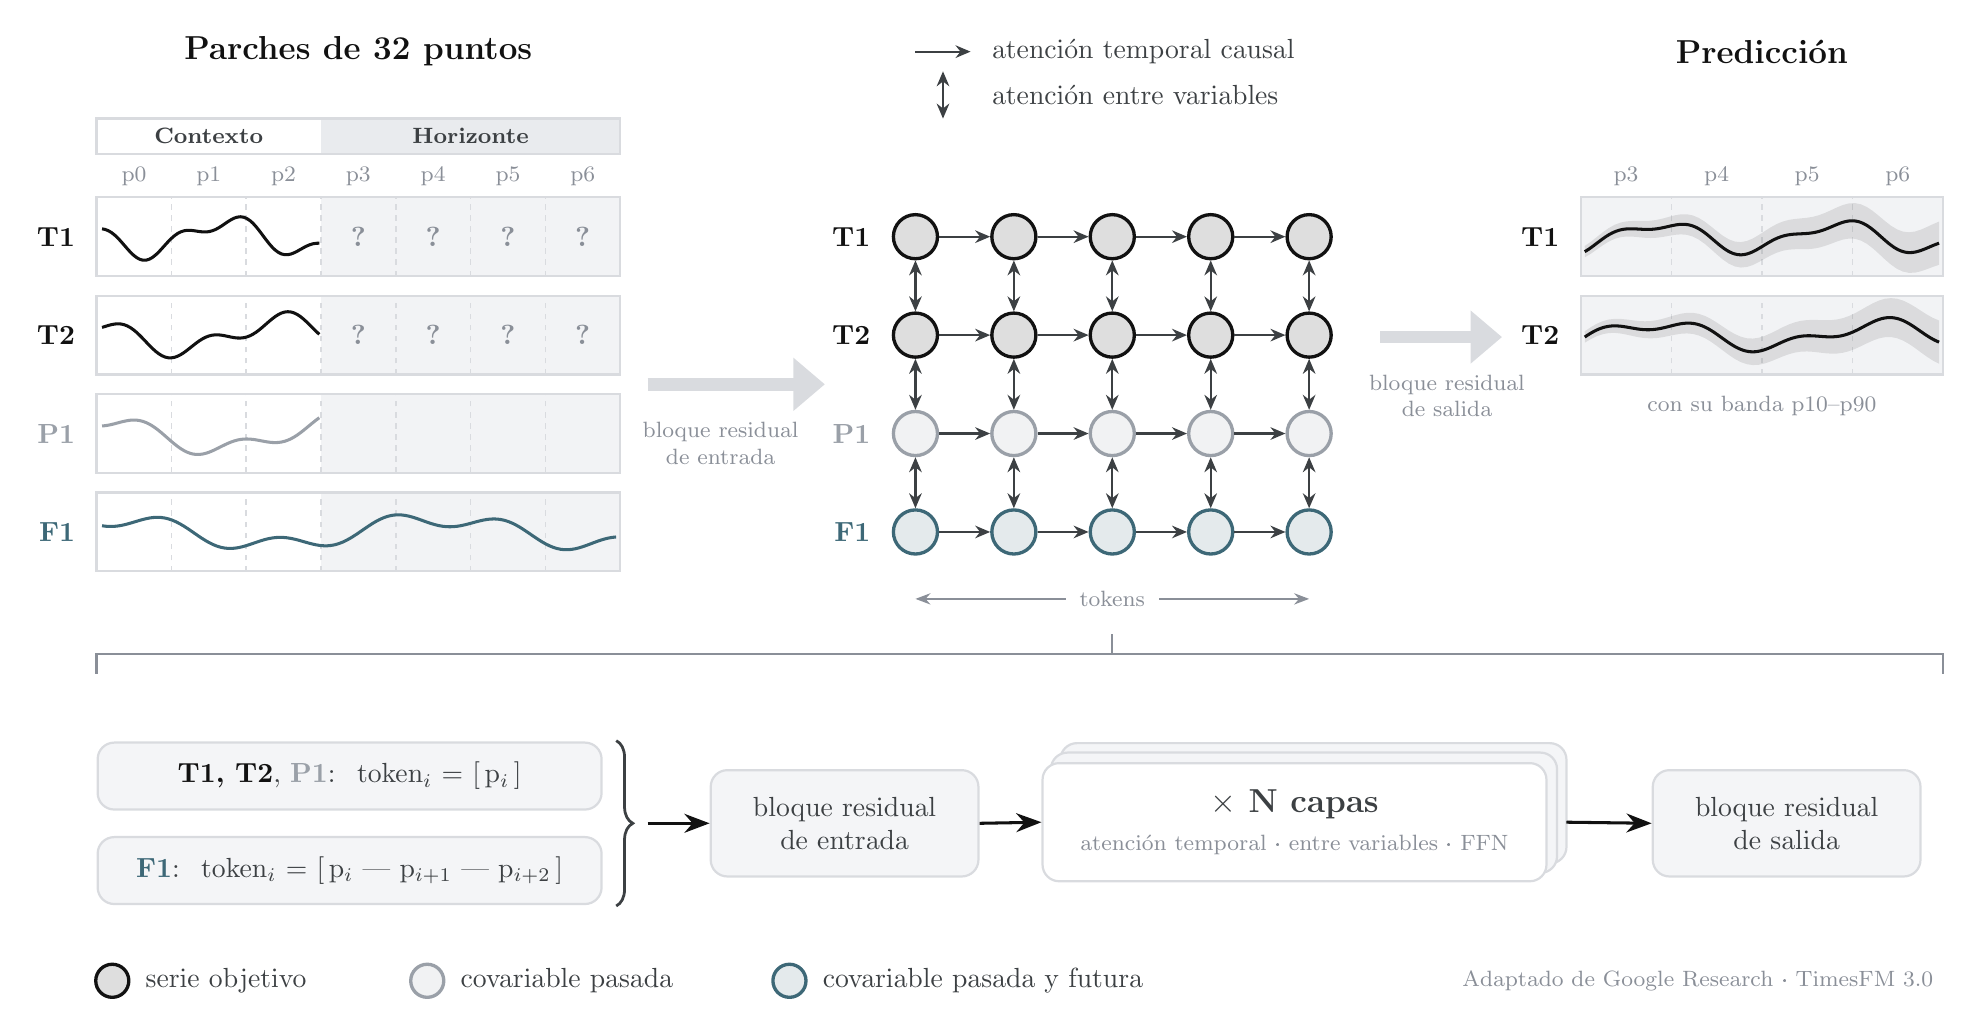
\begin{tikzpicture}[x=1cm,y=1cm]
  % Filas comunes a los tres paneles: T1, T2, P1, F1
  \def\yA{12.2}\def\yB{10.95}\def\yC{9.7}\def\yD{8.45}
  \def\H{0.5}                          % media altura de cada fila
  \def\PW{0.95}                        % ancho de un parche
  \def\XL{0.9}                         % borde izquierdo de los parches
  \pgfmathsetmacro{\XH}{\XL+3*\PW}     % donde empieza el horizonte
  \pgfmathsetmacro{\XR}{\XL+7*\PW}

  % --- Panel izquierdo: parches de contexto y horizonte ------------------------------------
  \node[ttl] at ({(\XL+\XR)/2},14.55) {Parches de 32 puntos};
  \fill[white] (\XL,13.25) rectangle (\XH,13.7);
  \fill[hzn] (\XH,13.25) rectangle (\XR,13.7);
  \draw[rule, line width=0.8pt] (\XL,13.25) rectangle (\XR,13.7);
  \node[font=\footnotesize\bfseries\color{ink2}] at ({(\XL+\XH)/2},13.475) {Contexto};
  \node[font=\footnotesize\bfseries\color{ink2}] at ({(\XH+\XR)/2},13.475) {Horizonte};
  \foreach \k in {0,...,6} \node[sm] at ({\XL+(\k+0.5)*\PW},12.97) {p\k};

  \foreach \y/\n/\c in {\yA/T1/tgt, \yB/T2/tgt, \yC/P1/pst, \yD/F1/fut} {
    \fill[hzn!60] (\XH,\y-\H) rectangle (\XR,\y+\H);
    \draw[rule, line width=0.8pt] (\XL,\y-\H) rectangle (\XR,\y+\H);
    \foreach \k in {1,...,6} \draw[rule, line width=0.6pt, dash pattern=on 2pt off 2pt] ({\XL+\k*\PW},\y-\H) -- ({\XL+\k*\PW},\y+\H);
    \node[lab, color=\c, anchor=east] at (\XL-0.15,\y) {\n};
  }
  % Series: las objetivo y la pasada solo en el contexto; la pasada y futura, también en el horizonte
  \draw[tgt, line width=1.1pt, smooth] plot[domain=0.97:3.73, samples=70] (\x,{\yA+0.2*sin(3.1*\x r)+0.1*sin(7.3*\x r+1)});
  \draw[tgt, line width=1.1pt, smooth] plot[domain=0.97:3.73, samples=70] (\x,{\yB+0.19*sin(2.4*\x r+0.5)+0.11*sin(6.1*\x r)});
  \draw[pst, line width=1.1pt, smooth] plot[domain=0.97:3.73, samples=70] (\x,{\yC+0.2*sin(1.9*\x r+2)+0.1*sin(5.2*\x r+0.3)});
  \draw[fut, line width=1.1pt, smooth] plot[domain=0.97:7.5, samples=140] (\x,{\yD+0.17*sin(1.5*\x r+1)+0.1*sin(4.4*\x r)});
  \foreach \y in {\yA,\yB} \foreach \k in {3,...,6} \node[font=\normalsize\bfseries\color{muted}] at ({\XL+(\k+0.5)*\PW},\y) {?};

  % --- Centro: tokens con atención temporal (→) y entre variables (↕) ----------------------
  \def\GX{11.3}\def\GP{1.25}
  \foreach \y/\n/\c in {\yA/T1/tgt, \yB/T2/tgt, \yC/P1/pst, \yD/F1/fut} {
    \node[lab, color=\c, anchor=east] at (\GX-0.45,\y) {\n};
    \foreach \k in {0,...,4} \node[tok, draw=\c, fill=\c!14] (n\n\k) at ({\GX+\k*\GP},\y) {};
    \foreach \k [evaluate=\k as \j using int(\k+1)] in {0,...,3} \draw[att] (n\n\k) -- (n\n\j);
  }
  \foreach \k in {0,...,4} {
    \draw[both] (nT1\k) -- (nT2\k);
    \draw[both] (nT2\k) -- (nP1\k);
    \draw[both] (nP1\k) -- (nF1\k);
  }
  \draw[att] (\GX,14.55) -- (\GX+0.7,14.55);
  \node[font=\normalsize\color{ink2}, anchor=west] at (\GX+0.85,14.55) {atención temporal causal};
  \draw[both] (\GX+0.35,13.7) -- (\GX+0.35,14.3);
  \node[font=\normalsize\color{ink2}, anchor=west] at (\GX+0.85,14.0) {atención entre variables};
  \draw[{Stealth[length=1.9mm]}-{Stealth[length=1.9mm]}, line width=0.8pt, muted] (\GX,7.6) -- (\GX+4*\GP,7.6);
  \node[fill=white, inner xsep=5pt, sm] at (\GX+2*\GP,7.6) {tokens};

  % Flechas entre paneles, con los bloques residuales
  \pgfmathsetmacro{\MY}{(\yA+\yD)/2}
  \draw[big] (\XR+0.35,\MY) -- (\GX-1.15,\MY);
  \node[sm, align=center] at ({(\XR+\GX)/2-0.6},\MY-0.75) {bloque residual\\de entrada};
  \pgfmathsetmacro{\XO}{\GX+4*\GP+0.9}
  \draw[big] (\XO,\MY+0.6) -- (\XO+1.55,\MY+0.6);
  \node[sm, align=center] at (\XO+0.85,\MY-0.15) {bloque residual\\de salida};

  % --- Panel derecho: la predicción de las series objetivo, con su banda --------------------
  \pgfmathsetmacro{\XP}{\XO+2.55}
  \def\QW{1.15}
  \pgfmathsetmacro{\XQ}{\XP+4*\QW}
  \node[ttl] at ({(\XP+\XQ)/2},14.55) {Predicción};
  \foreach \k in {3,...,6} \node[sm] at ({\XP+(\k-2.5)*\QW},12.97) {p\k};
  \foreach \y/\n in {\yA/T1, \yB/T2} {
    \fill[hzn!60] (\XP,\y-\H) rectangle (\XQ,\y+\H);
    \draw[rule, line width=0.8pt] (\XP,\y-\H) rectangle (\XQ,\y+\H);
    \foreach \k in {1,...,3} \draw[rule, line width=0.6pt, dash pattern=on 2pt off 2pt] ({\XP+\k*\QW},\y-\H) -- ({\XP+\k*\QW},\y+\H);
    \node[lab, color=tgt, anchor=east] at (\XP-0.15,\y) {\n};
  }
  \fill[ink, opacity=0.1] plot[domain=\XP+0.05:\XQ-0.05, samples=60] (\x,{\yA+0.17*sin(2.8*\x r)+0.07*sin(6*\x r)+0.07+0.045*(\x-\XP)})
        -- plot[domain=\XQ-0.05:\XP+0.05, samples=60] (\x,{\yA+0.17*sin(2.8*\x r)+0.07*sin(6*\x r)-0.07-0.045*(\x-\XP)}) -- cycle;
  \draw[tgt, line width=1.1pt, smooth] plot[domain=\XP+0.05:\XQ-0.05, samples=80] (\x,{\yA+0.17*sin(2.8*\x r)+0.07*sin(6*\x r)});
  \fill[ink, opacity=0.1] plot[domain=\XP+0.05:\XQ-0.05, samples=60] (\x,{\yB+0.15*sin(2.2*\x r+1)+0.08*sin(5.1*\x r)+0.07+0.045*(\x-\XP)})
        -- plot[domain=\XQ-0.05:\XP+0.05, samples=60] (\x,{\yB+0.15*sin(2.2*\x r+1)+0.08*sin(5.1*\x r)-0.07-0.045*(\x-\XP)}) -- cycle;
  \draw[tgt, line width=1.1pt, smooth] plot[domain=\XP+0.05:\XQ-0.05, samples=80] (\x,{\yB+0.15*sin(2.2*\x r+1)+0.08*sin(5.1*\x r)});
  \node[sm] at ({(\XP+\XQ)/2},\yB-\H-0.4) {con su banda p10--p90};

  % --- Abajo: cómo se forma cada token y la pila de capas ----------------------------------
  \draw[muted, line width=0.8pt] (\XL,6.65) -- (\XL,6.9) -- (\XQ,6.9) -- (\XQ,6.65);
  \draw[muted, line width=0.8pt] (\GX+2*\GP,6.9) -- (\GX+2*\GP,7.15);

  \node[blk, anchor=west, minimum width=6.4cm, minimum height=8.5mm] (ta) at (\XL,5.35)
    {\textcolor{tgt}{\textbf{T1, T2}}, \textcolor{pst}{\textbf{P1}}: \ token$_i$ = [\,p$_i$\,]};
  \node[blk, anchor=west, minimum width=6.4cm, minimum height=8.5mm] (tb) at (\XL,4.15)
    {\textcolor{fut}{\textbf{F1}}: \ token$_i$ = [\,p$_i$ | p$_{i+1}$ | p$_{i+2}$\,]};
  \draw[decorate, decoration={brace, amplitude=6pt}, line width=1pt, ink2] (\XL+6.6,5.8) -- (\XL+6.6,3.7);
  \node[blk, minimum width=3.4cm, minimum height=1.35cm] (in) at (\XL+9.5,4.75) {bloque residual\\de entrada};
  \draw[flow] (\XL+7.0,4.75) -- (in.west);
  \node[blk, minimum width=6.4cm, minimum height=1.5cm, anchor=south west, fill=white] (lay) at (\XL+12.0,4.0)
    {\textbf{\large $\times$ N capas}\\[2pt]{\footnotesize\color{muted} atención temporal · entre variables · FFN}};
  \begin{scope}[on background layer]
    \foreach \d in {0.24,0.12} \fill[soft, draw=rule, line width=0.8pt, rounded corners=6pt] ($(lay.south west)+(\d,\d)$) rectangle ($(lay.north east)+(\d,\d)$);
  \end{scope}
  \draw[flow] (in.east) -- (lay.west);
  \node[blk, minimum width=3.4cm, minimum height=1.35cm, anchor=west] (out) at (\XL+19.75,4.75) {bloque residual\\de salida};
  \draw[flow] ($(lay.east)+(0.24,0)$) -- (out.west);

  % Leyenda y fuente
  \def\ly{2.75}
  \node[tok, draw=tgt, fill=tgt!14, minimum size=4.2mm] at (\XL+0.2,\ly) {};
  \node[font=\normalsize\color{ink2}, anchor=west] at (\XL+0.5,\ly) {serie objetivo};
  \node[tok, draw=pst, fill=pst!14, minimum size=4.2mm] at (\XL+4.2,\ly) {};
  \node[font=\normalsize\color{ink2}, anchor=west] at (\XL+4.5,\ly) {covariable pasada};
  \node[tok, draw=fut, fill=fut!14, minimum size=4.2mm] at (\XL+8.8,\ly) {};
  \node[font=\normalsize\color{ink2}, anchor=west] at (\XL+9.1,\ly) {covariable pasada y futura};
  \node[sm, anchor=east] at (\XQ,\ly) {Adaptado de Google Research · TimesFM 3.0};
\end{tikzpicture}
\end{document}
